\documentclass{standalone}
\usepackage{tikz}
\usetikzlibrary{patterns, positioning}
\usepackage[sfdefault]{ClearSans} %% option 'sfdefault' activates Clear Sans as the default text font
\usepackage[T1]{fontenc}

\begin{document}
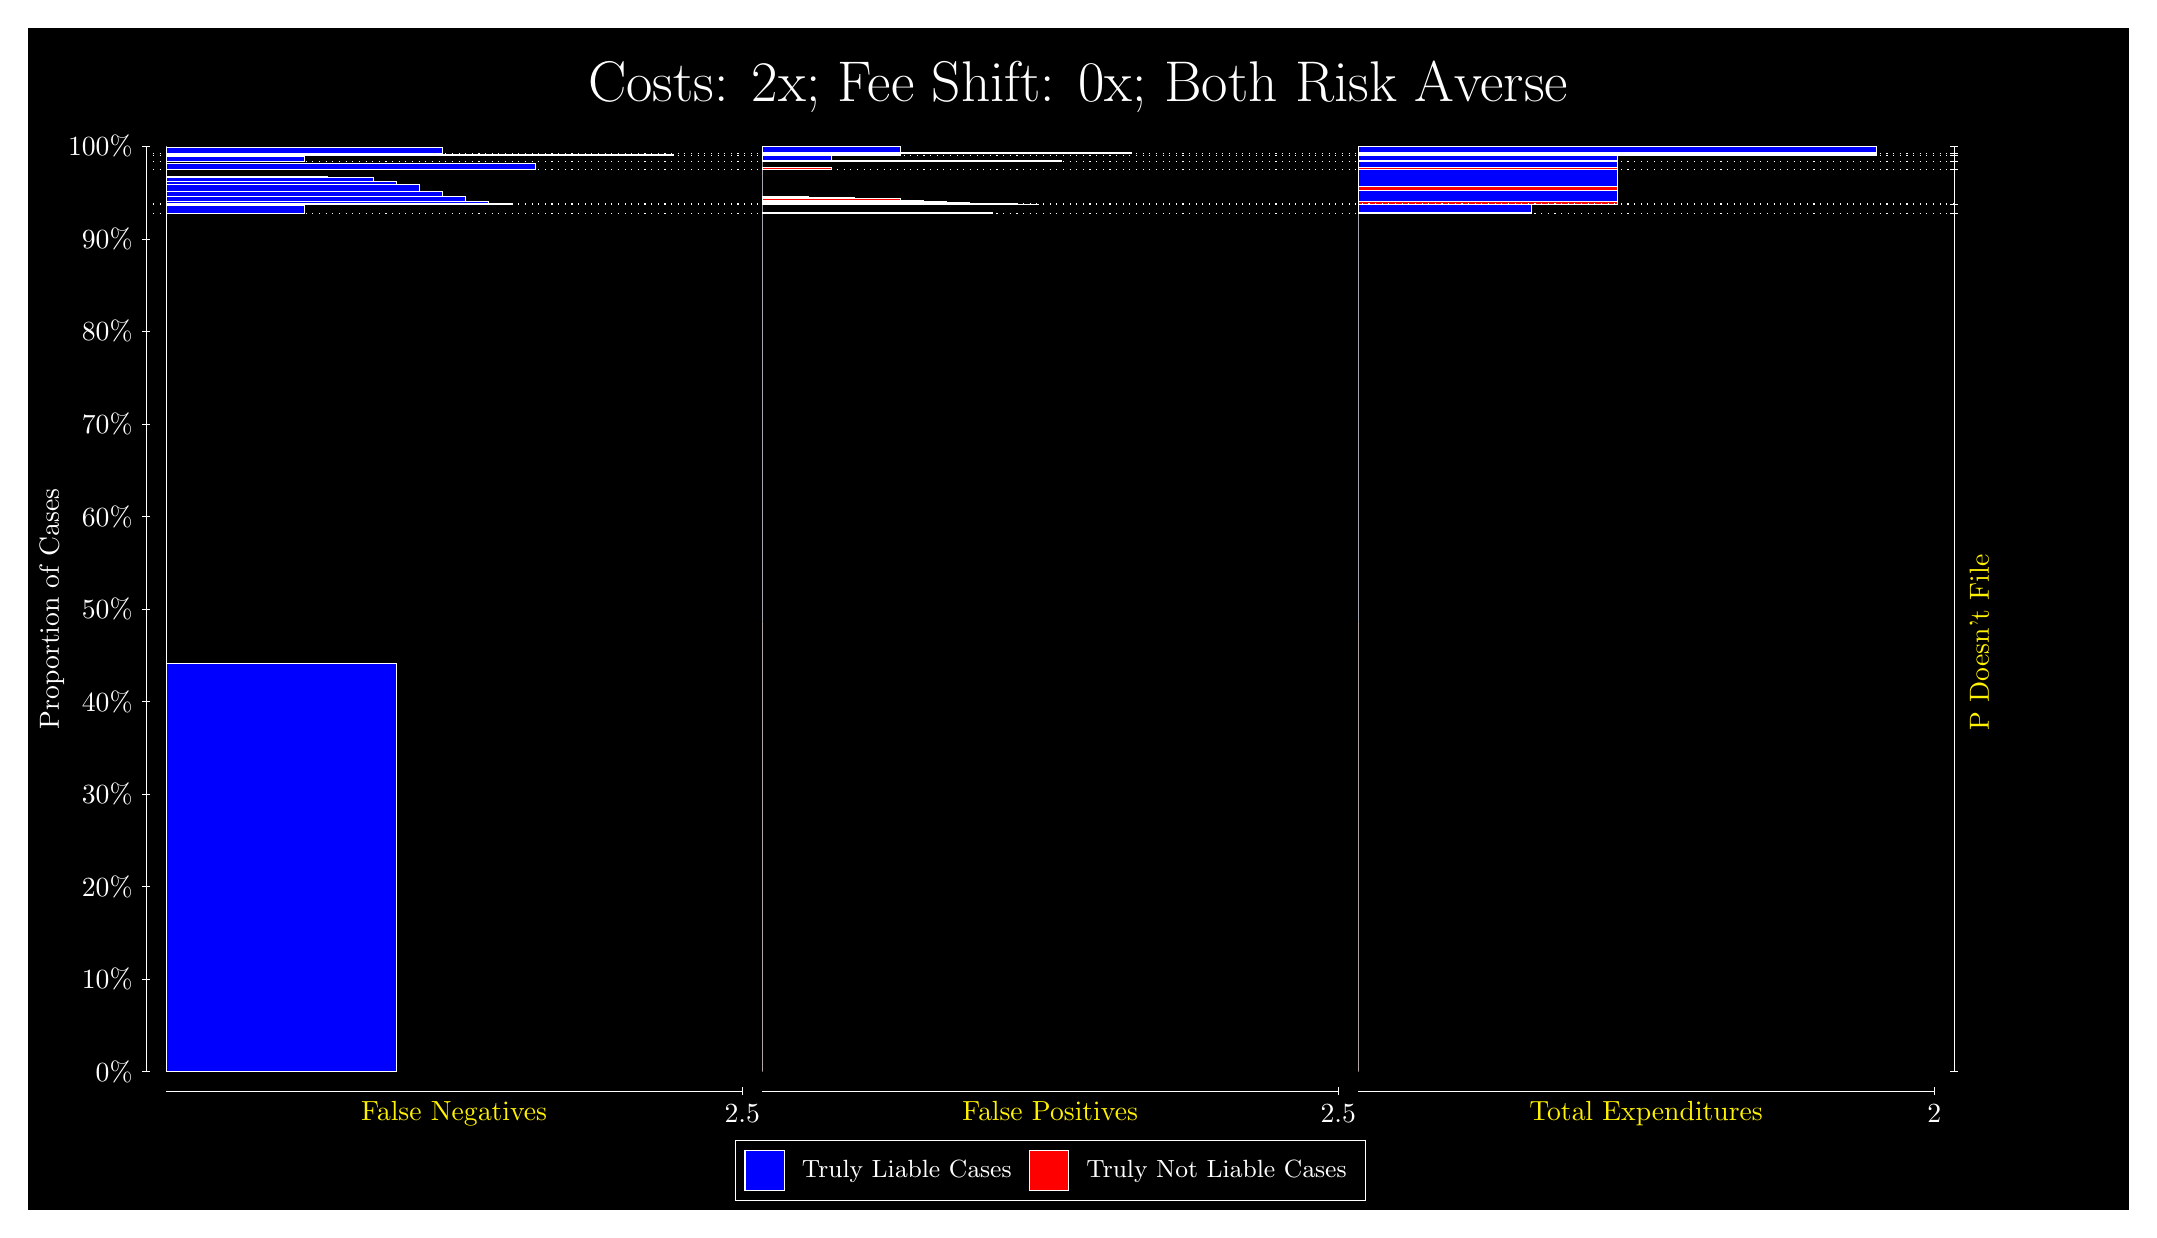
\begin{tikzpicture}
\draw[fill=black] (0,0) rectangle (26.667,15);
\draw[text=white] (0,13.5) rectangle (26.667,15) node[midway] {\huge Costs: 2x; Fee Shift: 0x; Both Risk Averse};
\draw[white, very thin] (1.5,1.75) -- (1.5,13.5);
\node[rotate=90, text=white, anchor=center] at (0.3, 7.625) {Proportion of Cases};
\draw[white, very thin] (1.45,1.75) -- (1.55,1.75);
\node[text=white, anchor=east] at (1.45, 1.75) {0\%};
\draw[white, very thin] (1.45,2.925) -- (1.55,2.925);
\node[text=white, anchor=east] at (1.45, 2.925) {10\%};
\draw[white, very thin] (1.45,4.1) -- (1.55,4.1);
\node[text=white, anchor=east] at (1.45, 4.1) {20\%};
\draw[white, very thin] (1.45,5.275) -- (1.55,5.275);
\node[text=white, anchor=east] at (1.45, 5.275) {30\%};
\draw[white, very thin] (1.45,6.45) -- (1.55,6.45);
\node[text=white, anchor=east] at (1.45, 6.45) {40\%};
\draw[white, very thin] (1.45,7.625) -- (1.55,7.625);
\node[text=white, anchor=east] at (1.45, 7.625) {50\%};
\draw[white, very thin] (1.45,8.8) -- (1.55,8.8);
\node[text=white, anchor=east] at (1.45, 8.8) {60\%};
\draw[white, very thin] (1.45,9.975) -- (1.55,9.975);
\node[text=white, anchor=east] at (1.45, 9.975) {70\%};
\draw[white, very thin] (1.45,11.15) -- (1.55,11.15);
\node[text=white, anchor=east] at (1.45, 11.15) {80\%};
\draw[white, very thin] (1.45,12.325) -- (1.55,12.325);
\node[text=white, anchor=east] at (1.45, 12.325) {90\%};
\draw[white, very thin] (1.45,13.5) -- (1.55,13.5);
\node[text=white, anchor=east] at (1.45, 13.5) {100\%};

\draw[white, very thin] (24.457,1.75) -- (24.457,13.5);
\draw[white, very thin] (24.407,1.75) -- (24.507,1.75);
\node[anchor=west] at (24.407, 1.75) {};
\draw[white, very thin] (24.407,12.65) -- (24.507,12.65);
\node[anchor=west] at (24.407, 12.65) {};
\draw[white, very thin] (24.407,12.768) -- (24.507,12.768);
\node[anchor=west] at (24.407, 12.768) {};
\draw[white, very thin] (24.407,13.205) -- (24.507,13.205);
\node[anchor=west] at (24.407, 13.205) {};
\draw[white, very thin] (24.407,13.312) -- (24.507,13.312);
\node[anchor=west] at (24.407, 13.312) {};
\draw[white, very thin] (24.407,13.382) -- (24.507,13.382);
\node[anchor=west] at (24.407, 13.382) {};
\draw[white, very thin] (24.407,13.412) -- (24.507,13.412);
\node[anchor=west] at (24.407, 13.412) {};
\draw[white, very thin] (24.407,13.5) -- (24.507,13.5);
\node[anchor=west] at (24.407, 13.5) {};

\draw[white, very thin, fill=blue] (1.75,1.75) rectangle (4.6775,6.9377);
\draw[white, very thin, fill=red] (1.75,6.9377) rectangle (1.75,12.65);
\draw[white, very thin, fill=blue] (1.75,12.65) rectangle (3.5065,12.752);
\draw[white, very thin, fill=red] (1.75,12.752) rectangle (1.75,12.768);
\draw[white, very thin, fill=blue] (1.75,12.768) rectangle (6.1413,12.78);
\draw[white, very thin, fill=blue] (1.75,12.78) rectangle (5.8486,12.801);
\draw[white, very thin, fill=blue] (1.75,12.801) rectangle (5.5558,12.86);
\draw[white, very thin, fill=blue] (1.75,12.86) rectangle (5.2631,12.932);
\draw[white, very thin, fill=blue] (1.75,12.932) rectangle (4.9703,13.014);
\draw[white, very thin, fill=blue] (1.75,13.014) rectangle (4.6775,13.059);
\draw[white, very thin, fill=blue] (1.75,13.059) rectangle (4.3848,13.103);
\draw[white, very thin, fill=blue] (1.75,13.103) rectangle (4.092,13.113);
\draw[white, very thin, fill=blue] (1.75,13.113) rectangle (3.7993,13.124);
\draw[white, very thin, fill=red] (1.75,13.124) rectangle (1.75,13.205);
\draw[white, very thin, fill=blue] (1.75,13.205) rectangle (6.4341,13.285);
\draw[white, very thin, fill=red] (1.75,13.285) rectangle (1.75,13.312);
\draw[white, very thin, fill=blue] (1.75,13.312) rectangle (3.5065,13.373);
\draw[white, very thin, fill=red] (1.75,13.373) rectangle (1.75,13.382);
\draw[white, very thin, fill=blue] (1.75,13.382) rectangle (8.1906,13.396);
\draw[white, very thin, fill=red] (1.75,13.396) rectangle (1.75,13.412);
\draw[white, very thin, fill=blue] (1.75,13.412) rectangle (5.2631,13.486);
\draw[white, very thin, fill=red] (1.75,13.486) rectangle (1.75,13.5);
\draw[white, very thin, fill=red] (9.3189,1.75) rectangle (9.3189,7.4626);
\draw[white, very thin, fill=blue] (9.3189,7.4626) rectangle (9.3189,12.65);
\draw[white, very thin, fill=red] (9.3189,12.65) rectangle (12.246,12.666);
\draw[white, very thin, fill=blue] (9.3189,12.666) rectangle (9.3189,12.768);
\draw[white, very thin, fill=red] (9.3189,12.768) rectangle (12.832,12.77);
\draw[white, very thin, fill=red] (9.3189,12.77) rectangle (12.539,12.771);
\draw[white, very thin, fill=red] (9.3189,12.771) rectangle (12.246,12.778);
\draw[white, very thin, fill=red] (9.3189,12.778) rectangle (11.954,12.786);
\draw[white, very thin, fill=red] (9.3189,12.786) rectangle (11.661,12.802);
\draw[white, very thin, fill=red] (9.3189,12.802) rectangle (11.368,12.817);
\draw[white, very thin, fill=red] (9.3189,12.817) rectangle (11.075,12.835);
\draw[white, very thin, fill=red] (9.3189,12.835) rectangle (10.783,12.843);
\draw[white, very thin, fill=red] (9.3189,12.843) rectangle (10.49,12.848);
\draw[white, very thin, fill=blue] (9.3189,12.848) rectangle (9.9044,12.86);
\draw[white, very thin, fill=blue] (9.3189,12.86) rectangle (9.6116,12.87);
\draw[white, very thin, fill=blue] (9.3189,12.87) rectangle (9.3189,13.205);
\draw[white, very thin, fill=red] (9.3189,13.205) rectangle (10.197,13.232);
\draw[white, very thin, fill=blue] (9.3189,13.232) rectangle (9.3189,13.312);
\draw[white, very thin, fill=red] (9.3189,13.312) rectangle (13.125,13.321);
\draw[white, very thin, fill=blue] (9.3189,13.321) rectangle (10.197,13.382);
\draw[white, very thin, fill=red] (9.3189,13.382) rectangle (11.075,13.398);
\draw[white, very thin, fill=blue] (9.3189,13.398) rectangle (9.3189,13.412);
\draw[white, very thin, fill=red] (9.3189,13.412) rectangle (14.003,13.426);
\draw[white, very thin, fill=blue] (9.3189,13.426) rectangle (11.075,13.5);
\draw[white, very thin, fill=red] (16.888,1.75) rectangle (16.888,7.4626);
\draw[white, very thin, fill=blue] (16.888,7.4626) rectangle (16.888,12.65);
\draw[white, very thin, fill=red] (16.888,12.65) rectangle (19.083,12.666);
\draw[white, very thin, fill=blue] (16.888,12.666) rectangle (19.083,12.768);
\draw[white, very thin, fill=red] (16.888,12.768) rectangle (20.181,12.797);
\draw[white, very thin, fill=blue] (16.888,12.797) rectangle (20.181,12.945);
\draw[white, very thin, fill=red] (16.888,12.945) rectangle (20.181,12.996);
\draw[white, very thin, fill=blue] (16.888,12.996) rectangle (20.181,13.205);
\draw[white, very thin, fill=red] (16.888,13.205) rectangle (20.181,13.232);
\draw[white, very thin, fill=blue] (16.888,13.232) rectangle (20.181,13.312);
\draw[white, very thin, fill=red] (16.888,13.312) rectangle (20.181,13.321);
\draw[white, very thin, fill=blue] (16.888,13.321) rectangle (20.181,13.382);
\draw[white, very thin, fill=red] (16.888,13.382) rectangle (23.475,13.398);
\draw[white, very thin, fill=blue] (16.888,13.398) rectangle (23.475,13.412);
\draw[white, very thin, fill=red] (16.888,13.412) rectangle (23.475,13.426);
\draw[white, very thin, fill=blue] (16.888,13.426) rectangle (23.475,13.5);
\draw[white, dotted] (1.5,12.65) -- (24.457,12.65);
\draw[white, dotted] (1.5,12.768) -- (24.457,12.768);
\draw[white, dotted] (1.5,13.205) -- (24.457,13.205);
\draw[white, dotted] (1.5,13.312) -- (24.457,13.312);
\draw[white, dotted] (1.5,13.382) -- (24.457,13.382);
\draw[white, dotted] (1.5,13.412) -- (24.457,13.412);
\draw[white, very thin] (1.75,1.5) -- (9.0689,1.5);
\node[text=yellow, anchor=north] at (5.4094, 1.5) {False Negatives};
\draw[white, very thin] (9.0689,1.45) -- (9.0689,1.55);
\node[text=white, anchor=north] at (9.0689, 1.45) {2.5};

\draw[white, very thin] (9.3189,1.5) -- (16.638,1.5);
\node[text=yellow, anchor=north] at (12.978, 1.5) {False Positives};
\draw[white, very thin] (16.638,1.45) -- (16.638,1.55);
\node[text=white, anchor=north] at (16.638, 1.45) {2.5};

\draw[white, very thin] (16.888,1.5) -- (24.207,1.5);
\node[text=yellow, anchor=north] at (20.547, 1.5) {Total Expenditures};
\draw[white, very thin] (24.207,1.45) -- (24.207,1.55);
\node[text=white, anchor=north] at (24.207, 1.45) {2};

\node[text=yellow, centered, rotate=90] at (24.777, 7.2001) {P Doesn't File};







\draw (12.978300999999998,1.5) node[draw=none] (baseCoordinate) {};
\begin{scope}[align=center]
        \matrix[scale=0.5, draw=white, below=0.5cm of baseCoordinate, nodes={draw}, column sep=0.1cm]{
            \node[rectangle, draw, minimum width=0.5cm, minimum height=0.5cm, fill=blue] {}; &
            \node[draw=none, font=\small, text=white] (B) {Truly Liable Cases}; &
            \node[rectangle, draw, minimum width=0.5cm, minimum height=0.5cm, fill=red] {}; &
            \node[draw=none, font=\small, text=white] (B) {Truly Not Liable Cases}; \\
            };
\end{scope}

\end{tikzpicture}
\end{document}